\documentclass[a4paper,11pt]{article}
\usepackage{graphicx}
\usepackage{amsmath}
\usepackage{hyperref}
\usepackage{caption}
\usepackage{subcaption}
\usepackage{float}
\usepackage[margin=0.55in]{geometry}

\title{Natural Language Processing Coursework \\ \large COMM061}
\author{Rohit Krishnan \\ Student ID:\ 6839323}
\date{\today}

\begin{document}

\maketitle

% \tableofcontents

\section{Introduction}\label{sec:introduction}
In this report, I present the results of my experimentation on
token classification for abbreviation and long form detection.
The task involves labelling abbreviations and their corresponding
long forms using a BIO tagging scheme. The dataset used for this
coursework is derived from biomedical literature, specifically
from the PLOS journal articles.

\section{Dataset Analysis and Visualization}\label{sec:dataset-analysis}
\subsection{Dataset Overview}
The dataset consists of 50k labelled tokens with the following labels: B-O,
B-AC, I-AC, B-LF, I-LF.\ Each token is accompanied by its corresponding
part-of-speech (POS) tag.

\subsection{Data Visualization}
\begin{figure}[H]
	\centering
	\begin{minipage}[t]{0.48\textwidth}
		\centering
		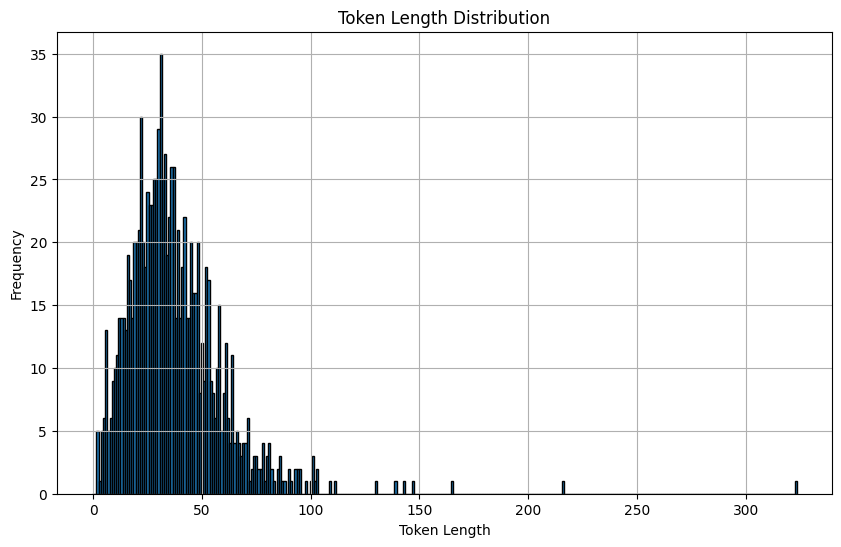
\includegraphics[width=\textwidth]{./assets/token_len_hist.png}
		\caption{Visualization of the token length of samples from the PLOD-CW dataset}\label{fig:token_len_hist}
	\end{minipage}
	\hfill
	\begin{minipage}[t]{0.48\textwidth}
		\centering
		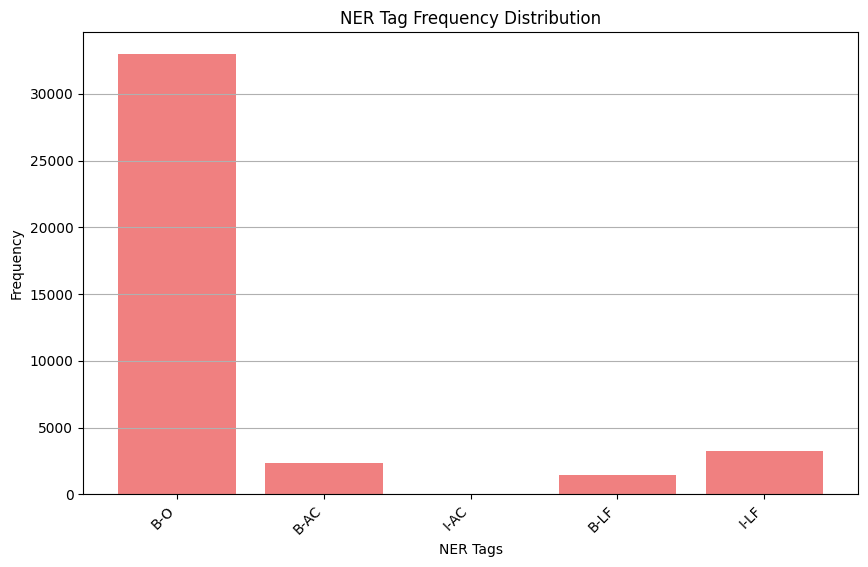
\includegraphics[width=\textwidth]{./assets/ner_tag_freq.png}
		\caption{Visualization of the NER tag frequency in the dataset}\label{fig:ner_tag_freq}
	\end{minipage}
\end{figure}

The histogram of token lengths shows that most tokens have lengths ranging from
0 to 50, with a peak around the 20\-30 token range. The I-LF tag, which marks
tokens inside a long form, also shows a modest frequency, indicating that long
forms are often multi-token phrases.

\begin{figure}[H]
	\centering
	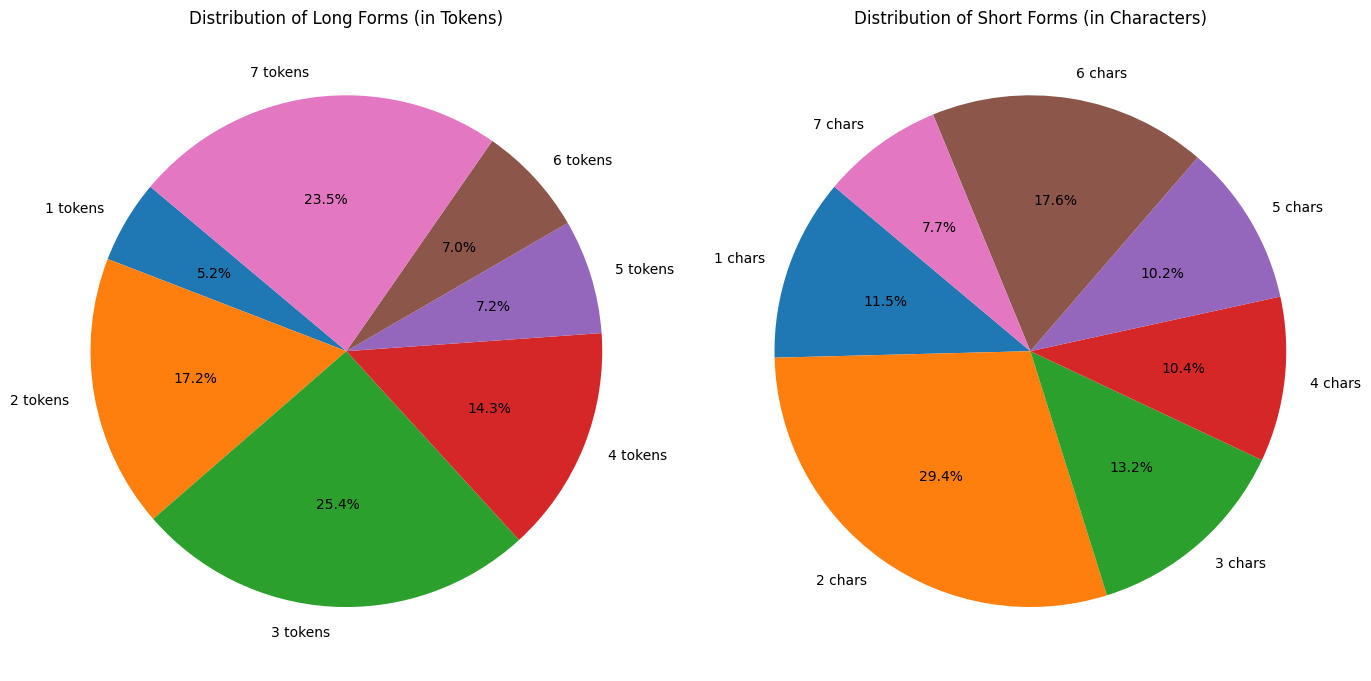
\includegraphics[width=6.5in]{./assets/dist_lf_abbr.png}
	\caption{Distributions of long forms in no.\ of tokens (left) and short forms in no.\ of characters (right)}\label{fig:dist_lf_abbr}
\end{figure}

Abbreviations are typically concise, with a preference for short character
sequences. Long forms tend to be multi-word phrases, with a tendency toward 3
to 7 tokens.

\subsection{Observations}

These visualizations suggest that the model needs to be robust in handling
imbalanced data, capturing contextual information across multiple tokens, and
efficiently processing sequences of varying lengths. Pre-trained language
models like BERT or RoBERTa, which are adept at capturing contextual
relationships, are well-suited for this task.

The distribution also implies that padding strategies need to be efficient.
Since most sequences are short, using a fixed-length input size for training
could lead to a lot of padding, which might waste computational resources and
potentially introduce noise.

The dataset's characteristics imply that evaluation metrics should focus not
only on overall accuracy but also on precision, recall, and F1-score for the
minority classes (B-AC, B-LF, I-LF). This will ensure that the model is
performing well on the key task of identifying abbreviations and long forms,
rather than just predicting the majority class correctly. Since there are no
instances of the I-AC class, dropping the class alltogether would help in
improving the model's performance.

\section{Experimentation and Evaluation}\label{sec:experimentation}
\subsection{Experiment 1: Fine-Tuning Sequence Classification Models}
Several pre-trained language models were fine-tuned, using the PLOD-CW dataset.
The models were chosen based on their popularity and effectiveness in sequence
classification tasks. Apart from BERT and RoBERTa that are widely accepted
models for sequence classification, I also experimented with models pre-trained
on biomedical data \underline{\textbf{TODO:cite}}

\begin{figure}[H]
	\centering
	\begin{minipage}[t]{0.48\textwidth}
		\centering
		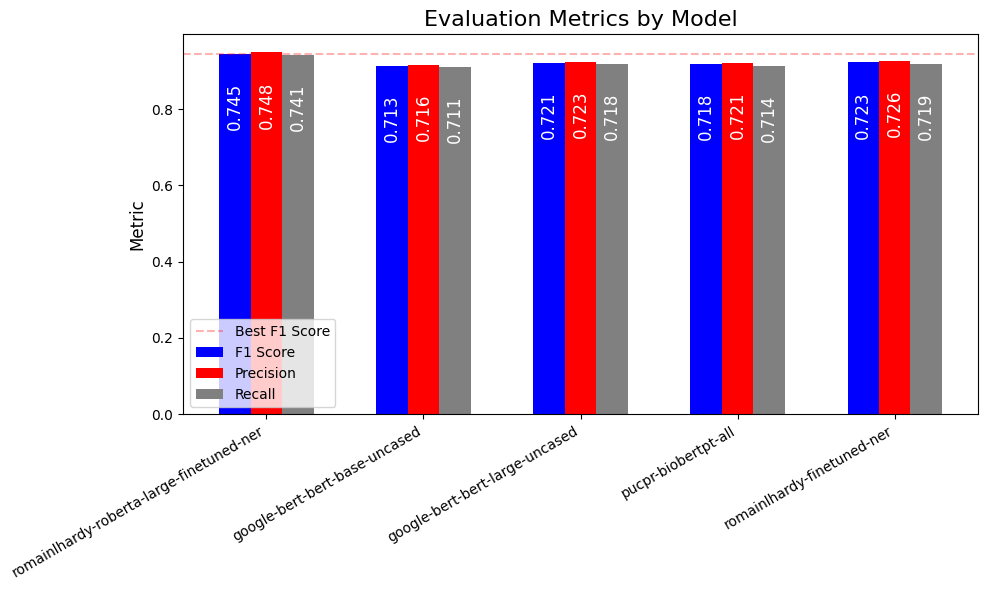
\includegraphics[width=\textwidth]{./assets/model_f1.png}
		\caption{Visualization of the token length of samples from the PLOD-CW dataset}\label{fig:model_f1}
	\end{minipage}
	\hfill
	\begin{minipage}[t]{0.48\textwidth}
		\centering
		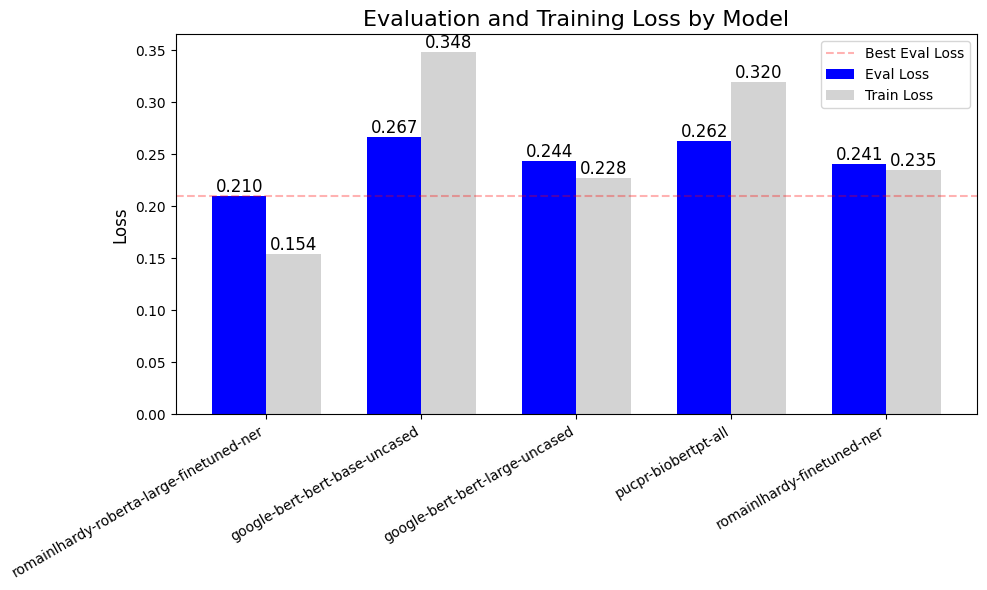
\includegraphics[width=\textwidth]{./assets/model_train_eval_loss.png}
		\caption{Visualization of the NER tag frequency in the dataset}\label{fig:model_losses}
	\end{minipage}
\end{figure}

\begin{table}[H]
	\centering
	\caption{Training results for commonly used models}
	\begin{tabular}{|c|c|c|c|c|}
		\hline
		\textbf{Model}                         & \textbf{Batch Size} & \textbf{Epochs} & \textbf{F1 Score $\uparrow$} & \textbf{Eval Loss $\downarrow$} \\ \hline
		google-bert/bert-base-uncased          & 8                   & 20              & 0.913                        & 0.267                           \\ \hline
		pucpr/biobertpt-all                    & 8                   & 20              & 0.918                        & 0.262                           \\ \hline
		google-bert/bert-large-uncased         & 8                   & 20              & 0.921                        & 0.244                           \\ \hline
		romainlhardy/finetuned-ner (bert-base) & 8                   & 20              & 0.923                        & 0.241                           \\ \hline
		\textbf{roberta-large-finetuned-ner}   & 8                   & 20              & \textbf{0.945}               & \textbf{0.210}                  \\ \hline
	\end{tabular}\label{tab:experiment_results}
\end{table}

\subsection{Experiment 2: Hyperparameter Optimization}
Of all the runs, \textbf{romainlhardy/roberta-large-finetuned-ner} showed the most promising
results. I performed hyperparameter optimization using Optuna for the
\textbf{romainlhardy/roberta-large-finetuned-ner} model as it had the highest F1 score.


\begin{figure}[H]
	\centering
	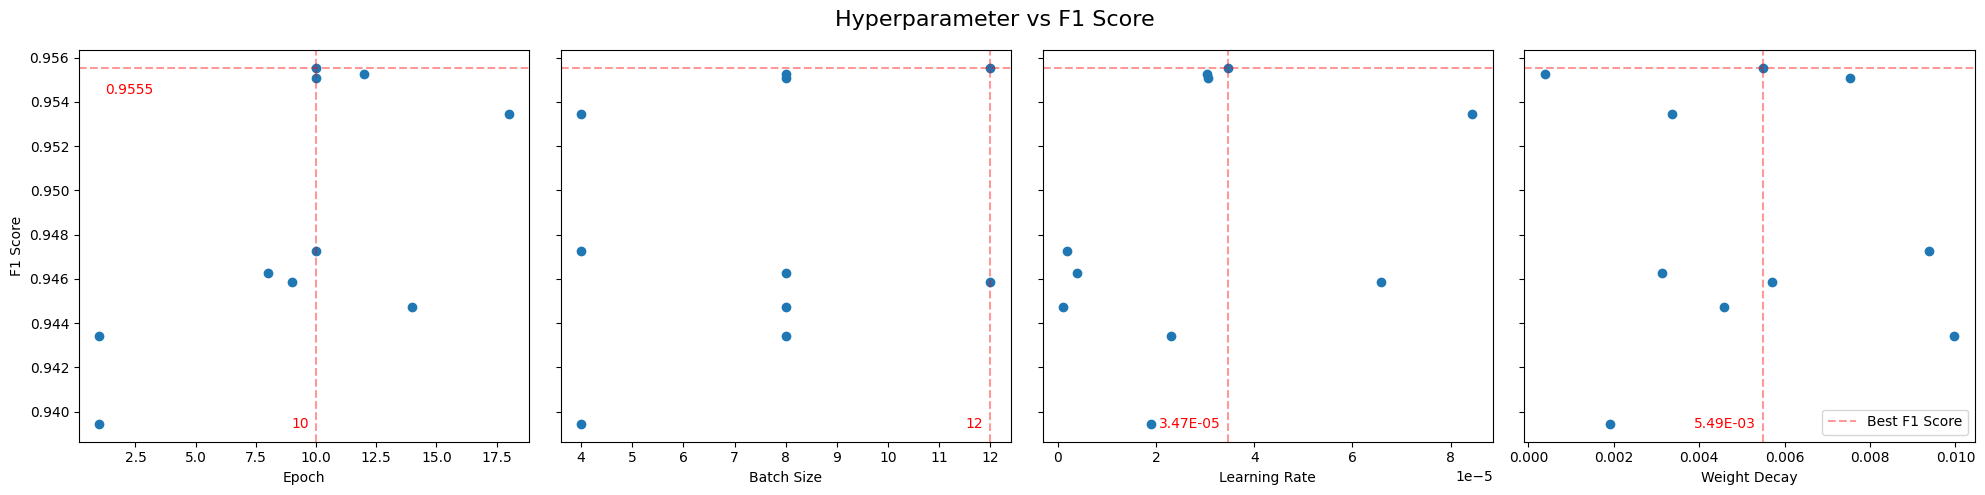
\includegraphics[width=6.5in]{./assets/hparam.png}
	\caption{Hyperparameter optimization using Optuna}\label{fig:hparam}
\end{figure}


\begin{table}[H]
	\centering
	\caption{Hyperparameter Optimization Results for google-bert/bert-large-uncased}
	\begin{tabular}{|c|c|c|c|c|}
		\hline
		\textbf{Learning Rate} & \textbf{Batch Size} & \textbf{Epochs} & \textbf{F1 Score $\uparrow$} & \textbf{Eval Loss $\downarrow$} \\ \hline
		0.000008               & 12                  & 20              & 0.9062                       & 0.2880                          \\ \hline
		0.000016               & 12                  & 10              & 0.9202                       & 0.2509                          \\ \hline
		0.000003               & 4                   & 10              & 0.9357                       & 0.2625                          \\ \hline
		0.000003               & 8                   & 10              & 0.9322                       & 0.2320                          \\ \hline
		0.000072               & 12                  & 20              & 0.9066                       & 0.2694                          \\ \hline
		0.000010               & 8                   & 15              & 0.9352                       & 0.3304                          \\ \hline
		0.000004               & 8                   & 10              & 0.9342                       & 0.2344                          \\ \hline
		0.000006               & 12                  & 20              & 0.9376                       & 0.3362                          \\ \hline
		0.000011               & 4                   & 15              & \textbf{0.9394}              & 0.4690                          \\ \hline
		0.000002               & 4                   & 20              & 0.9337                       & \textbf{0.2736}                 \\ \hline
	\end{tabular}\label{tab:hyperparam_results_all}
\end{table}

\subsection{Testing and Error Analysis}
[Include confusion matrices, classification reports, and any error analysis conducted.]

\section{Testing and Deployment}\label{sec:testing-deployment}
\subsection{Best Results and Adjustments}
[Discuss the best results obtained, any adjustments made, and their impact.]

\subsection{Model Evaluation and Efficiency}
[Evaluate the overall performance of the models and discuss the trade-offs between accuracy and efficiency.]

\subsection{Model Serving Options}
[Research and discuss different model serving options, and justify the choice made for deployment.]

\subsection{API/Web-Service Deployment}
We deployed the best-performing model as an API endpoint using [framework or
		tool used]. The architecture is simple, running locally on the machine with the
following key components:

\begin{itemize}
	\item Model loading and inference.
	\item API endpoint setup using [tool used, e.g., Flask].
	\item Input/output handling for sequence classification.
\end{itemize}

\begin{figure}[H]
	\centering
	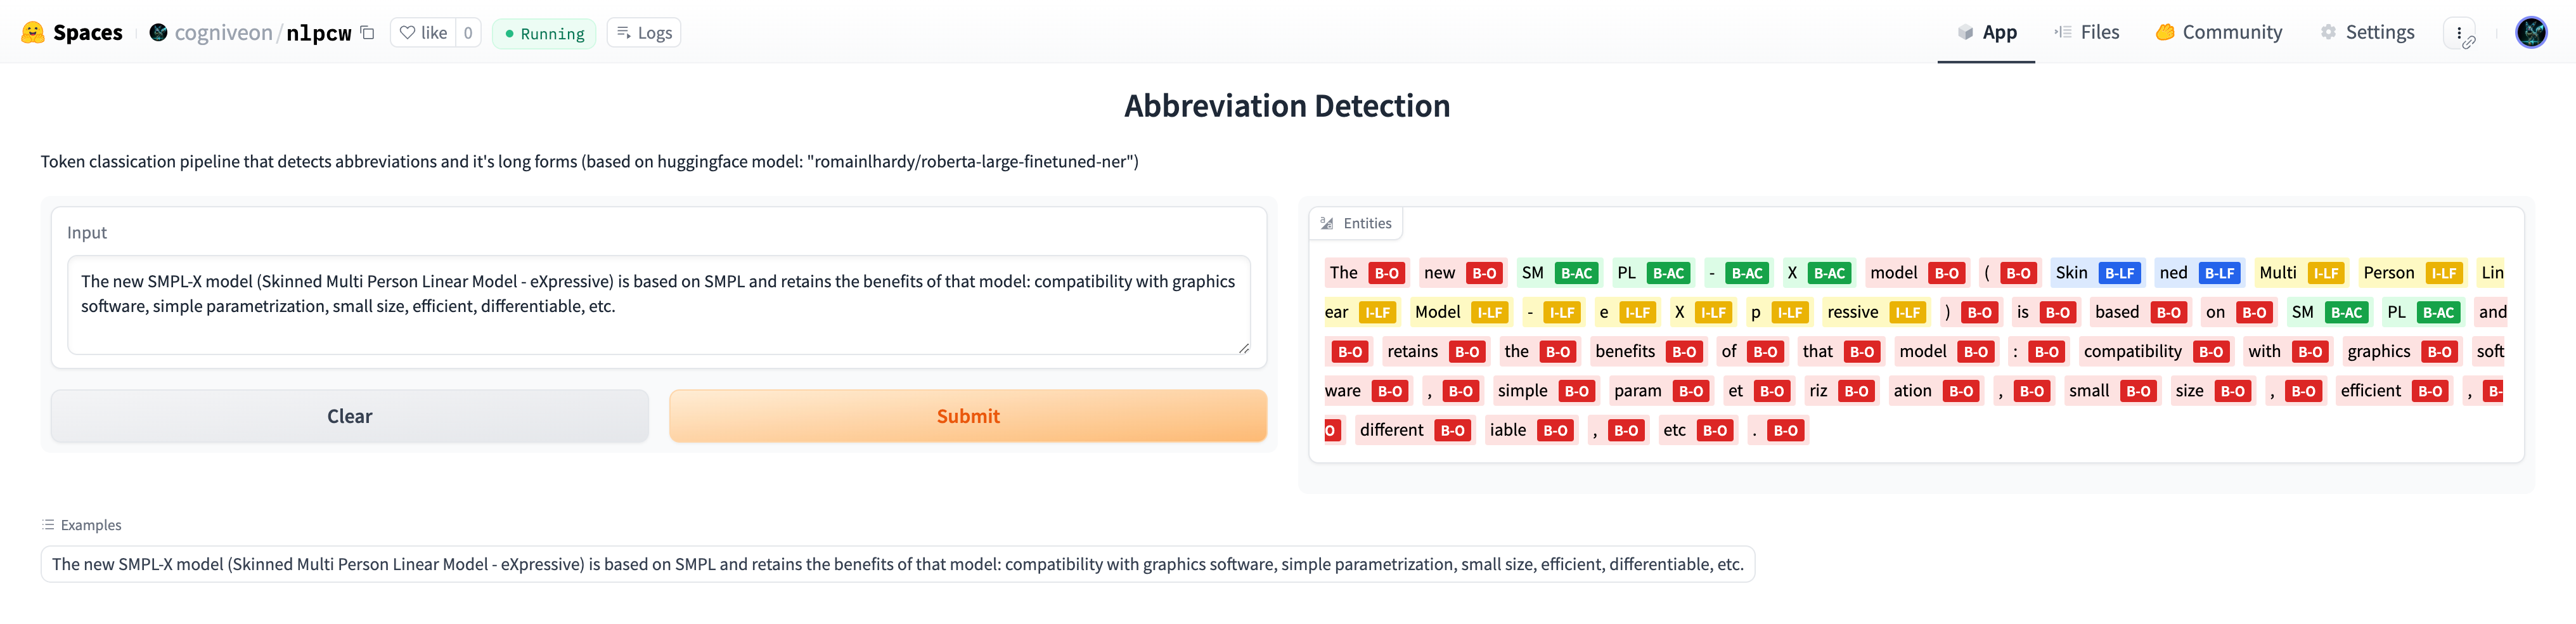
\includegraphics[width=\textwidth]{./assets/demo.png}
	\caption{Screenshot of the API response.}\label{fig:api-screenshot}
\end{figure}

\section{Conclusion}\label{sec:conclusion}
In this report, we demonstrated the process of fine-tuning pre-trained models for sequence classification, hyperparameter optimization, and deploying the model as an API service. The results show that [summarize your key findings and the effectiveness of your approach].

\section{References}\label{sec:references}
[Include all the references for papers, code, and resources you used.]

\end{document}
